%
% ---------- header -----------------------------------------------------------
%
% project       kaneton
%
% license       kaneton
%
% file          /home/mycure/kaneton/view/lecture/philosophy/philosophy.tex
%
% created       julien quintard   [wed may 16 19:41:40 2007]
% updated       julien quintard   [fri may 21 16:20:45 2010]
%

%
% ---------- setup ------------------------------------------------------------
%

%
% path
%

\def\path{../..}

%
% template
%

%
% ---------- header -----------------------------------------------------------
%
% project       kaneton
%
% license       kaneton
%
% file          /home/mycure/kaneton/view/template/lecture.tex
%
% created       julien quintard   [wed may 16 18:17:26 2007]
% updated       julien quintard   [sun may 18 23:23:40 2008]
%

%
% class
%

\documentclass[8pt]{beamer}

%
% packages
%

\usepackage{pgf,pgfarrows,pgfnodes,pgfautomata,pgfheaps,pgfshade}
\usepackage[T1]{fontenc}
\usepackage{colortbl}
\usepackage{times}
\usepackage{amsmath,amssymb}
\usepackage{graphics}
\usepackage{graphicx}
\usepackage{color}
\usepackage{xcolor}
\usepackage[english]{babel}
\usepackage{enumerate}
\usepackage[latin1]{inputenc}
\usepackage{verbatim}
\usepackage{aeguill}

%
% style
%

\usepackage{beamerthemesplit}
\setbeamercovered{dynamic}

%
% verbatim stuff
%

\definecolor{verbatimcolor}{rgb}{0.00,0.40,0.00}

\makeatletter

\renewcommand{\verbatim@font}
  {\ttfamily\footnotesize\selectfont}

\def\verbatim@processline{
  {\color{verbatimcolor}\the\verbatim@line}\par
}

\makeatother

%
% -
%

\renewcommand{\-}{\vspace{0.4cm}}

%
% date
%

\date{\today}

%
% logos
%

\pgfdeclareimage[interpolate=true,width=34pt,height=18pt]
                {epita}{\path/logo/epita}
\pgfdeclareimage[interpolate=true,width=49pt,height=18pt]
                {upmc}{\path/logo/upmc}
\pgfdeclareimage[interpolate=true,width=25pt,height=18pt]
                {lse}{\path/logo/lse}

\newcommand{\logos}
  {
    \pgfuseimage{epita}
  }

%
% institute
%

\institute
{
  \inst{1} kaneton microkernel project
}

%
% table of contents at the beginning of each section
%

\AtBeginSection[]
{
  \begin{frame}<beamer>
   \frametitle{Outline}
    \tableofcontents[current]
  \end{frame}
}

%
% table of contents at the beginning of each subsection
%

\AtBeginSubsection[]
{
  \begin{frame}<beamer>
   \frametitle{Outline}
    \tableofcontents[current,currentsubsection]
  \end{frame}
}


%
% title
%

\title{Philosophy}

%
% document
%

\begin{document}

%
% title frame
%

\begin{frame}
  \titlepage
\end{frame}

%
% outline frame
%

\begin{frame}
  \frametitle{Outline}

  \tableofcontents
\end{frame}

%
% motivation
%

\section{Motivation}

% 1)

\begin{frame}
  \frametitle{Education}

  \term{kaneton} was created when students at \name{EPITA} needed a support
  for system courses.

  \-

  kaneton was therefore designed with an \term{education} objective in mind.
\end{frame}

% 2)

\begin{frame}
  \frametitle{Simplicity}

  In the spirit of education, kaneton was designed to be as \term{simple},
  \term{clear} and \term{understandable} as possible.

  \-

  More specifically, many things were \term{abstract}ed so that students
  could focus on what was important for their curriculum.
\end{frame}

% 3)

\begin{frame}
  \frametitle{Portability}

  Today's computing world is synonym of \term{heterogeneity}.

  \-

  kaneton was designed to support multiple hardware components from the
  ground up.
\end{frame}

% 4)

\begin{frame}
  \frametitle{Modernity}

  kaneton was also designed with \term{modernity} in mind, providing features
  such as \term{safety}, \term{security} and so forth through the microkernel
  model but also \term{distributed computing} capabilities.

  \-

  Indeed, kaneton authors did not want to design and implement another
  boring UNIX-like.
\end{frame}

%
% design
%

\section{Design}

% 1)

\begin{frame}
  \frametitle{Introduction}

  This section discusses the design decisions that have a significant
  impact on the singularity of kaneton.
\end{frame}

% 2)

\begin{frame}
  \frametitle{Microkernel}

  \name{kaneton} differs from many operating system kernels in the way its
  architecture is \term{microkernel}-based.

  \-

  The microkernel architecture has been chosen because it provides
  \term{safety} guarantees. Indeed, whenever a component crashes, it can be
  relaunched unlike monolithic-based kernels which crash every time a
  driver has a problem.

  \-

  Besides, the microkernel architecture is propitious to \term{security} by
  respecting the \name{least privilege principle} since every component only
  has access to its own data.
\end{frame}

% 3)

\begin{frame}
  \frametitle{Portability}

  The microkernel is then split into logically separated units depending on
  their relation to the underlying hardware.

  \-

  Thus, the \term{core} contains the functionalities that are independent
  from the hardware also known as \name{machine-independent}.

  \-

  On the other hand, the code related to the hardware, also known as
  \name{machine-dependent}, is contained in the \term{machine} component.

  \-

  These terms were introduced in order to make it easier to communicate
  about the different components of the kernel.
\end{frame}

% 4)

\begin{frame}
  \frametitle{Core}

  The core is composed of \term{manager}s, every manager being
  responsible for a specific \term{object}.

  \-

  An object can be an event, a region of physical memory, a security token
  and so on. Note that there is no relation between object-oriented programming
  and kaneton objects.

  \-

  Furthermore, managers must not be considered as being isolated entities.
  Indeed, some managers are intrusive in the way they directly access another
  manager's data structures, as shown next.
\end{frame}

% 5)

\begin{frame}
  \frametitle{Managers}

  \begin{figure}[h]
    \begin{center}
      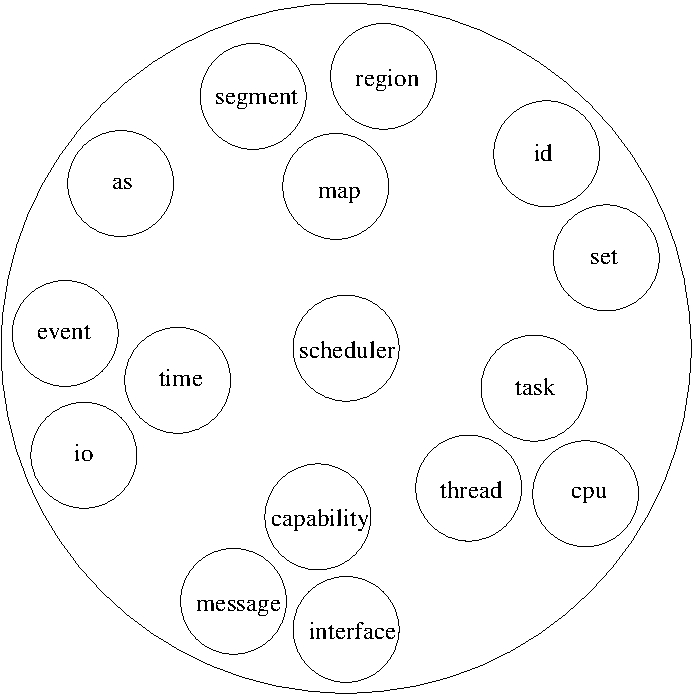
\includegraphics[scale=0.5]{\path/figures/managers-organisation.pdf}
    \end{center}
  \end{figure}
\end{frame}

% 6)

\begin{frame}
  \frametitle{Managers}

  Managers can be classified in categories depending on the type of object
  they are responsible for, which are described in detail below.

  \-

  The \term{segment}, \term{region} and \term{as} managers are responsible for
  the memory entities, respectively the areas of physical memory (not to be
  confound with \name{ia32} segments), the areas of virtual memory and
  the address spaces.

  \-

  The \term{event}, \term{io} and \term{time} deal with asynchronous events
  while \term{task}, \term{thread}, \term{cpu} and \term{scheduler} provide
  functionalities for execution contexts.


  \-

  The \term{message}, \term{capability} and \term{interface} managers
  provide communication capabilities.

  \-

  Finally, the \term{id} and \term{set} managers abstract the notions of
  object identification and storage in order for kernel developers to easily
  work with data structures.
\end{frame}

% 7)

\begin{frame}
  \frametitle{Machine}

  The machine is once again split into three subcomponents: \term{platform},
  \term{architecture} and \term{glue}.

  \-

  The \name{platform} contains everything related to the \name{BSP - Board
  Support Package} such as the \name{PIC - Programmable Interrupt Controller},
  the \name{PIT - Programmable Interval Timer} \etc{}.

  \-

  Likewise the \name{architecture} contains everything related to the
  microprocessor.

  \-

  Finally, the \name{glue} component makes it easy to couple a platform with
  an architecture. Indeed, depending on the couple, calls related to the
  core's time manager, for instance, may be redirected to the platform
  which contains the \name{PIT} or to the architecture which embeds a
  specific timer.
\end{frame}

% 8)

\begin{frame}
  \frametitle{Modules}

  The kernel also contains often-non-portable additional components known
  as \term{modules}.

  \-

  Modules provide other functionalities such as a way to display information
  within the kernel until the microkernel's server responsible for the
  console is launched.

  \-

  Another module known as \name{forward} is in charge of forwarding all the
  displayed information to the serial controller so that it can be retrieved
  by another computer. Such a module is very helpful for debugging, especially
  from within an emulator.
\end{frame}

% 9)

\begin{frame}
  \frametitle{Library}

  A \term{library} is also provided which contains common standard
  functionalities such as copying memory, dealing with strings, printing
  formatted information and so forth.
\end{frame}

% 10)

\begin{frame}
  \frametitle{Layers}

  \begin{figure}[h]
    \begin{center}
      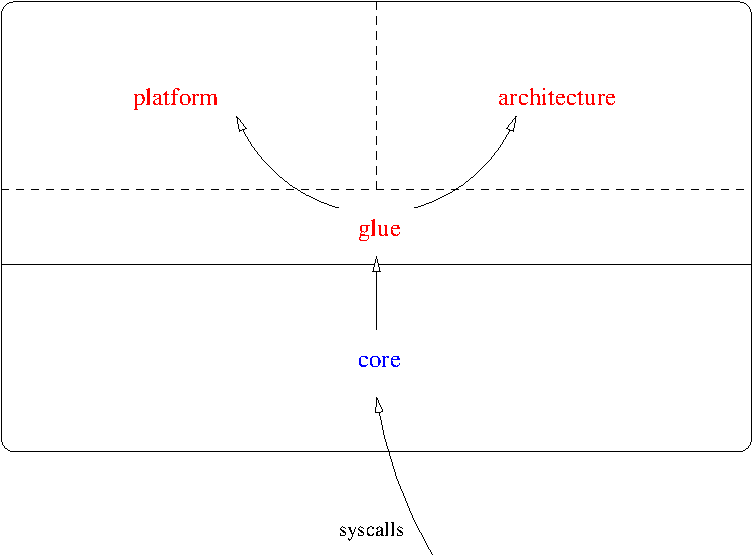
\includegraphics[scale=0.5]{\path/figures/kernel-layers.pdf}
    \end{center}
  \end{figure}
\end{frame}

% 11)

\begin{frame}[containsverbatim]
  \frametitle{Hierarchy}

  You can find all these components in the hierarchy:

  \begin{verbatim}
    kaneton/
      core/
        as/
        capability/
        [...]
      machine/
        architecture/
          ia32/
          mips64/
          [...]
        platform/
          ibm-pc/
          octane/
          [...]
        glue/
          ibm-pc.ia32/
          octane.mips64/
          [...]
      library/
      modules/
        console/
        forward/
        [...]
      include/
        [...]
  \end{verbatim}
\end{frame}

%
% implementation
%

\section{Implementation}

% 1)

\begin{frame}
  \frametitle{Introduction}

  This section discusses the implementation details that have a significant
  impact on the system.
\end{frame}

% 2)

\begin{frame}
  \frametitle{Interface}

  Every manager provides an \term{identical} interface composed of functions
  such as \code{initialize()}, \code{clean()}, \code{dump()} for the manager's
  management and \code{reserve()}, \code{release()}, \code{show()},
  \code{give()} \etc{} for the objects it is responsible for.

  \-

  Therefore, it is extremely easy for everyone to understand what a manager
  does given its consistent interface.
\end{frame}

% 3)

\begin{frame}
  \frametitle{Genericity}

  Let's recall that the \name{core} managers are independent of the underlying
  hardware. Therefore, the managers consider the received arguments in a
  \term{generic} way.

  \-

  For instance, the \name{ia32} architecture considers virtual memory as
  being composed of \name{pages} of $4096$ bytes.

  \-

  However, although the \name{region} manager provides a machine-independent
  virtual memory representation, the manager accepts addresses and sizes
  that are not aligned on $4096$.

  \-

  It is therefore the \name{machine}'s, and more presicely the
  \name{architecture}'s, responsability to reject unaligned calls.
\end{frame}

% 4)

\begin{frame}
  \frametitle{Set}

  Since students are not interested in writing data management code and
  since many kernel components require such a functionality, kaneton was
  designed to integrate a \term{set} manager.

  \-

  The set manager provides an \term{easy and transparent way} to
  \term{store data} since the underlying data structure can be changed by
  modifying a single parameter: linked-list, tree, array and so on.

  \-

  The set manager is composed of itself and set implementations such as ll,
  array, stack, bpt \etc{}

  \-

  First a set can be created with, for instance,
  \code{set\_reserve(ll, sizeof(t\_element), \&id)} for a linked-list. From
  this point, the set manager can be used to manipulate the freshly created
  set by passing the received identifier.

  \-

  Note that nothing is known of the underlying implementation and that
  the interface does not change should it be a balanced tree, a linked list
  or an array.
\end{frame}

% 5)

\begin{frame}
  \frametitle{Set}

  \begin{figure}[h]
    \begin{center}
      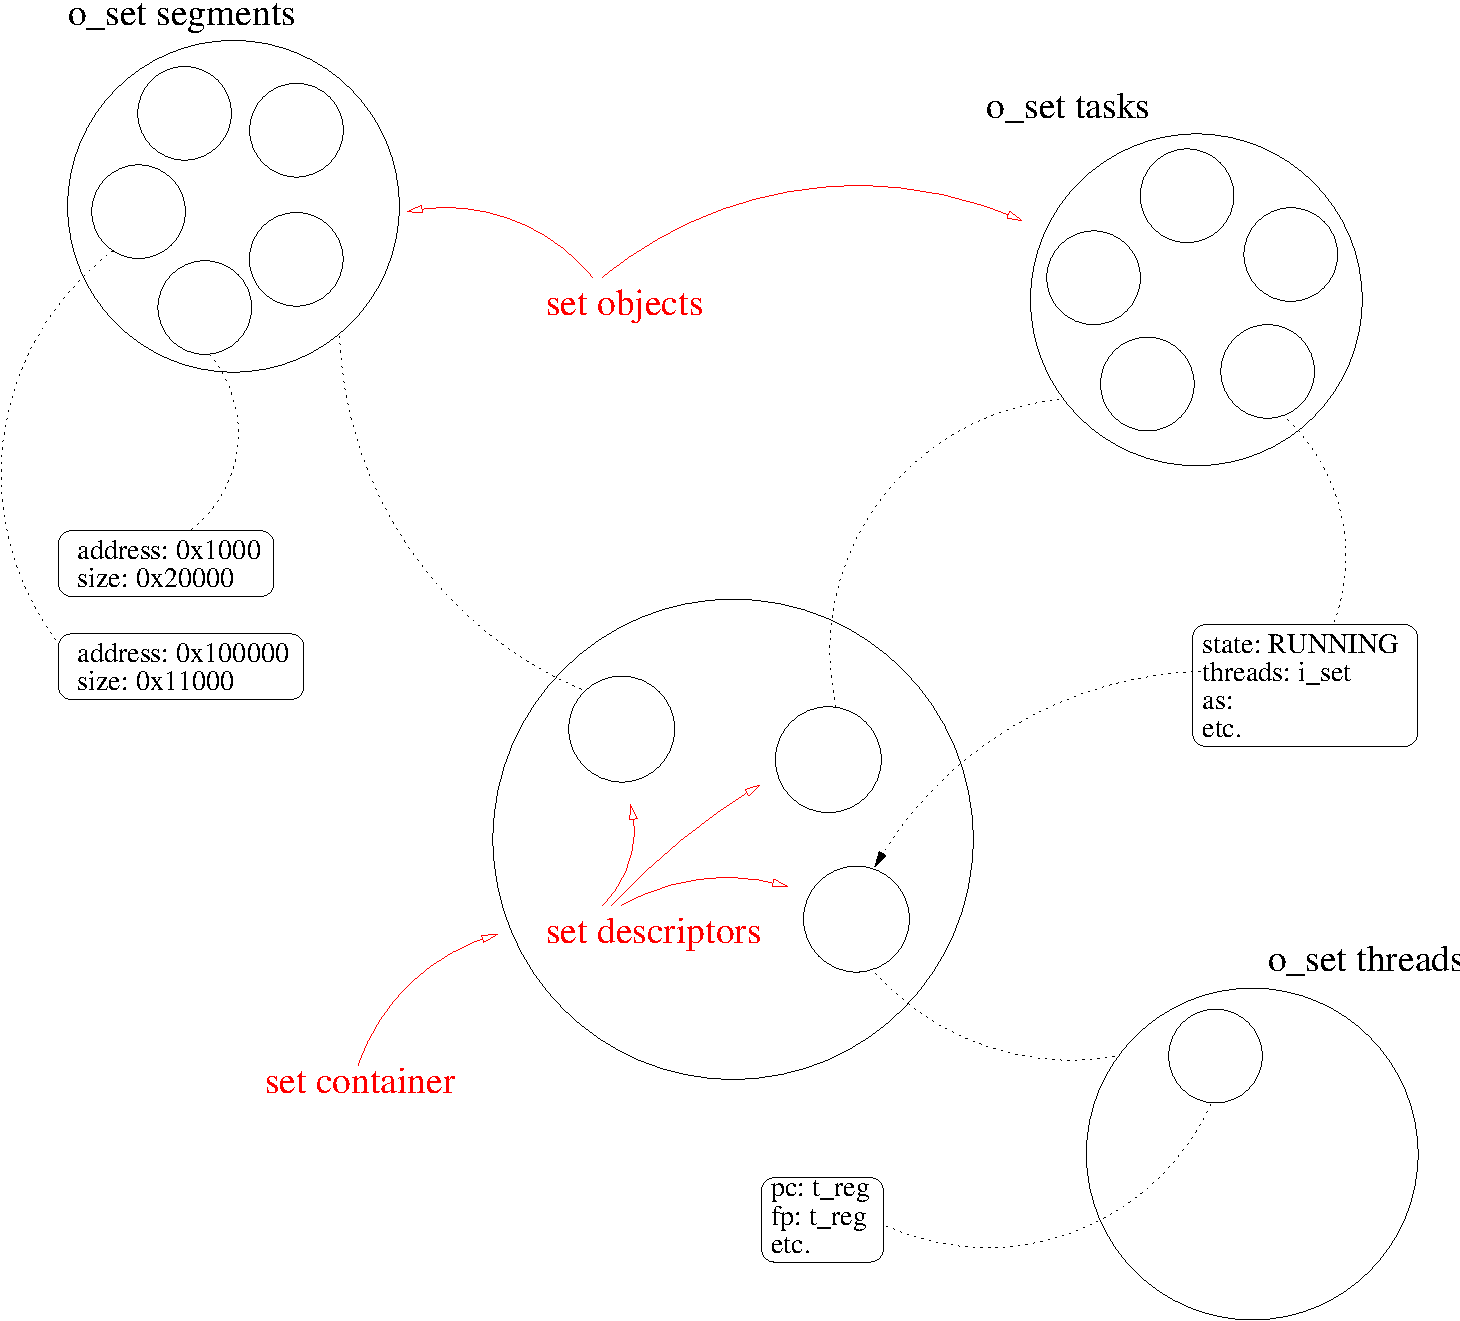
\includegraphics[scale=0.3]{\path/figures/sets-organisation.pdf}
    \end{center}
  \end{figure}
\end{frame}

% 6)

\begin{frame}
  \frametitle{Overhead}

  Note that the set manager probably introduces a \term{performance
  overhead} but since kaneton is not meant to become a real operating
  system kernel, this is not that important.
\end{frame}

% 7)

\begin{frame}
  \frametitle{Specific Physical Memory Management}

  All operating system kernels provide a physical memory manager.

  \-

  However, since all the other manager rely on this manager, the physical
  \term{memory manager} is \term{often} very \term{static}, relying on an
  extremely simple and specific data structure such as a bitmap.

  \-

  Since the objectives includes simplicity and modernity, kaneton's physical
  memory manager, known as the segment manager, was designed to rely on the
  set manager for storing data, very much as any other kaneton manager.

  \-

  Since the segment manager relies on the set manager which needs to allocate
  memory through \code{malloc()} which again will call the segment manager
  whenever it runs out of memory, a mutual dependency problem will arise.

  \-

  To prevent and delay this problem, kaneton relies on a \term{survival area}.
  This area is reserved by the boot loader and passed to the kernel then
  to \code{malloc()} so that this area can cover every memory allocation
  until the kernel is ready to operate fully.

  \-

  Note that this solution is not perfect since the size of the survival area
  must be guessed.
\end{frame}

% 8)

\begin{frame}
  \frametitle{Boot Loader}

  Following the kaneton objectives, the \name{core} must not contain any
  hardware-related source code, hence not assembly code.

  \-

  Therefore, kaneton designers decided to concentrate all the hardware-related
  setup in the boot loader so that the kernel is launched to operate in
  an \term{already operational environment}.

  \-

  The boot loader thus takes care to set up the virtual memory, to relocate
  the kernel code and stack where it should depending on the machine---for
  instance above the \name{DMA - Direct Memory Access} zone, to pass the
  pre-allocated segments and regions in a static array-like data structure,
  but also to pass the ready-to-launch first server.
\end{frame}

% 9)

\begin{frame}[containsverbatim]
  \frametitle{Init Structure}

  \begin{verbatim}
    t_paddr                       mem;
    t_psize                       memsz;

    t_paddr                       kcode;
    t_psize                       kcodesz;

    t_paddr                       scode;
    t_psize                       scodesz;
    t_vaddr                       slocation;
    t_vaddr                       sentry;

    t_paddr                       init;
    t_psize                       initsz;

    t_inputs*                     inputs;
    t_psize                       inputssz;
    t_uint32                      nsegments;
    s_segment*                    segments;
    t_psize                       segmentssz;

    t_uint32                      nregions;
    s_region*                     regions;
    t_psize                       regionssz;

    t_paddr                       kstack;
    t_psize                       kstacksz;

    t_paddr                       alloc;
    t_psize                       allocsz;
  \end{verbatim}
\end{frame}

% 10)

\begin{frame}
  \frametitle{Address Spaces}

  Whenever a system calls occur, the kernel is woken up by handling the
  syscall interrupt. Note that, at this point, the kernel evolves in the
  calling process' address space.

  \-

  If the kernel decides to allocate a new memory page, this will imply
  updating the page directory and tables.

  \-

  If the execution is given back to the process, then another process is
  scheduled which in turn perform a system call. If the kernel tries to
  access the data in the newly allocated page, the kernel will crash
  because, in this process' address space, the page directory and tables have
  not been modified to take it into account.

  \-

  Some kernels, including the \name{LSE/OS} propagate the modifications to
  all the other address spaces while the \name{Linux} kernel handles this
  problem by mirror-mapping all the physical memory.
\end{frame}

% 11)

\begin{frame}
  \frametitle{Address Spaces}

  In kaneton, a more \term{elegant solution} has been adopted consisting
  in mapping a single kernel page in each address space. This page contains
  the code for the interrupt handler. This code basically performs a single
  operation: switch the address space to the kernel's so that the following
  operations are all performed in the kernel environment.

  \-

  Unfortunately but obviously, this design choice has a drastic impact on
  the kernel performance since every system call implies switching the
  address space hence flushing the caches.
\end{frame}

\end{document}
